\begin{titlepage}
\date{}
\begin{figure}
\centering
\includegraphics[scale=0.35]{figures/KTH_Logo.png}
\end{figure}
\title{
\vspace{-1cm}
\textsc{DD2425 - Robotics and Autonomous Systems}
\\
\vspace{0.5cm}
\textsc{Group 6}\\
{\large \today}
\begin{center}
\rule{\linewidth}{0.5mm}
\textbf{Project Report}
\rule{\linewidth}{0.5mm}
\end{center}
}
\maketitle
\vspace{-2cm}
\begin{figure}[h]
\centering
\begin{minipage}[b]{0.5\linewidth}
                \begin{flushleft}
\normalsize{
\emph{Authors}\\
\vspace{0.5cm}
Carlos \textsc{Gálvez del Postigo} \\
Mathias \textsc{Lindblom} \\
Tingyu \textsc{Liu} \\
Gundars \textsc{Kalns}
}
\end{flushleft}
\end{minipage}
\qquad
\quad
\begin{minipage}[b]{0.4\linewidth}
                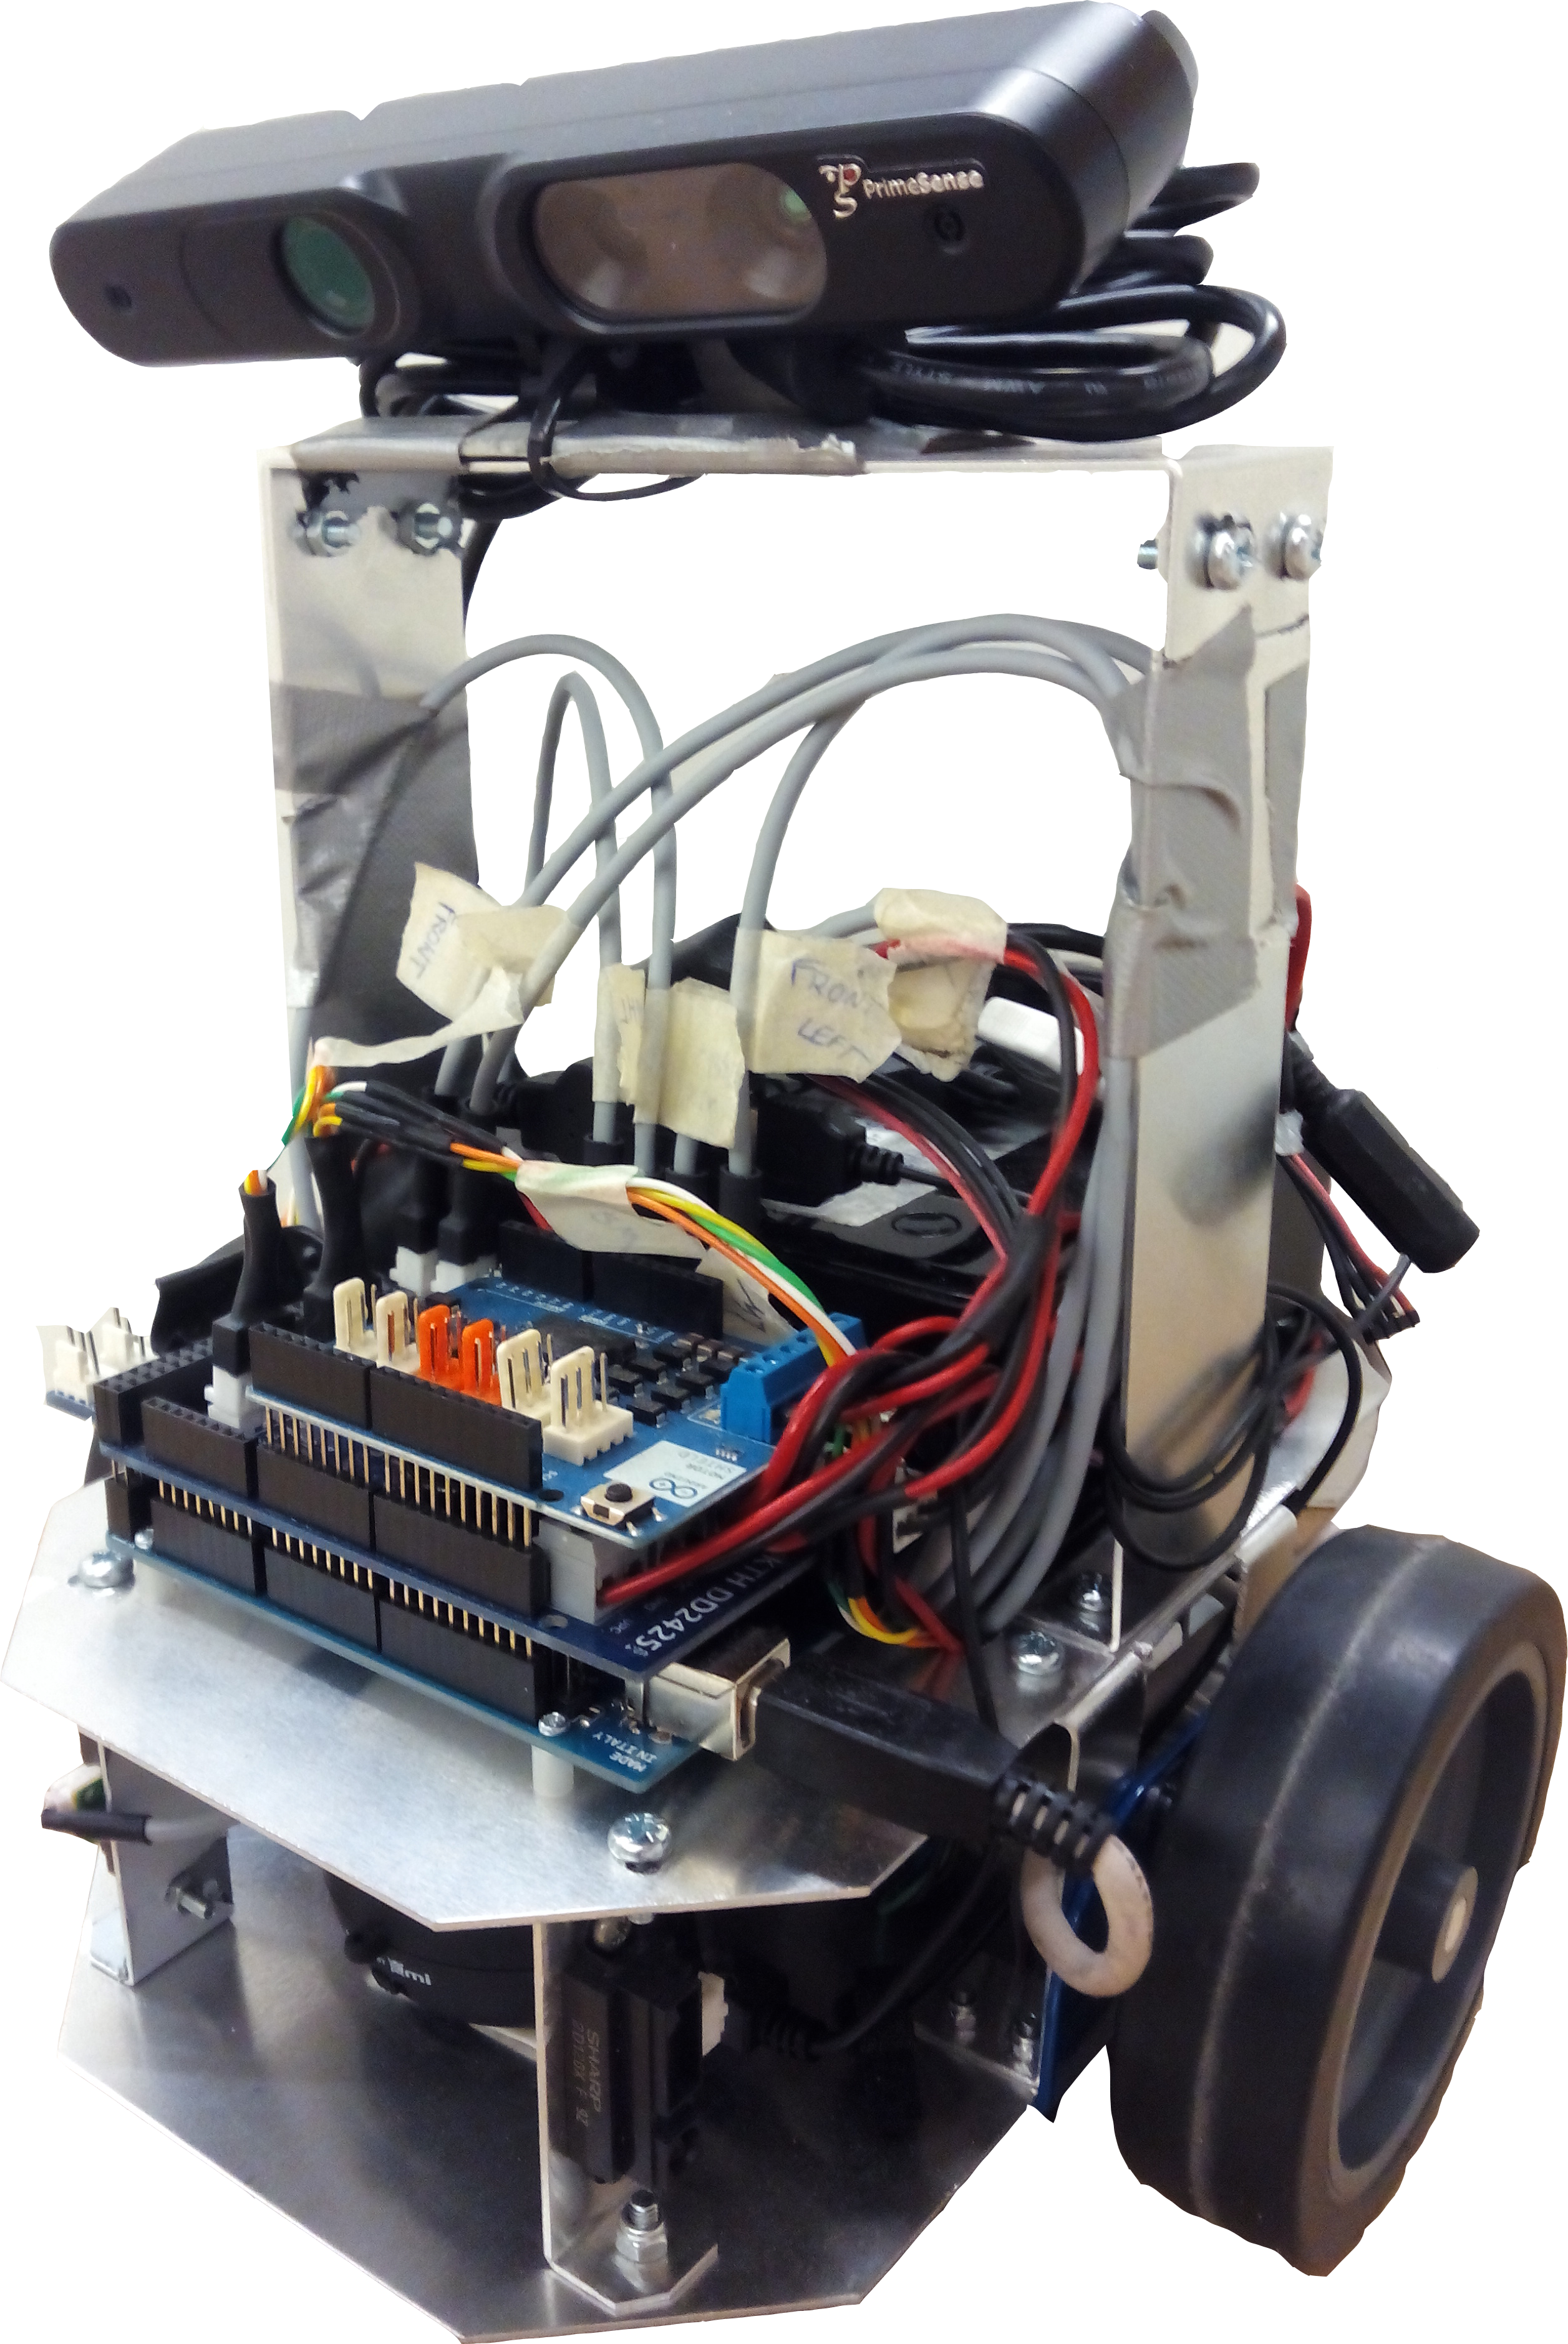
\includegraphics[width=0.6\linewidth]{figures/robot_title.png}
\end{minipage}
\end{figure}
\vspace{1cm}
\thispagestyle{empty}
\begin{abstract}
This report describes the work done for the Robotics and Autonomous Systems project. The task consisted on designing a robot that would be able to autonomously explore a maze, avoid obstacles, detected and identify objects and build a map as it navigates. In addition, on a second run, it had to be able to "fetch" the objects as fast as possible using the previously acquired knowledge. The robot was tested in the laboratory and in a contest with satisfactory results. Finally, a performance analysis and some conclusions summarize this report. 
\end{abstract}
\end{titlepage}